%情報処理学会全国大会原稿テンプレート ver. 1.2

\documentclass[uplatex,twocolumn]{jsarticle}
\usepackage[top=30mm,bottom=25mm,left=20mm,right=20mm]{geometry}
\usepackage[T1]{fontenc}
\usepackage{txfonts}
\usepackage[expert,deluxe]{otf}
\usepackage[dvipdfmx,hiresbb]{graphicx}
\usepackage[dvipdfm]{hyperref}
\usepackage{pxjahyper}
\usepackage{multicol}
\usepackage{here}
\setlength{\columnsep}{7mm}

\title{\vspace{-10mm}Twitter発言の分析によるWebサービス障害の影響調査\footnotemark[0]}
\author{\large{岩瀬 翔\footnotemark[2]\qquad 矢吹 太朗}\\千葉工業大学 社会システム科学部 プロジェクトマネジメント学科\footnotemark[3]}
\date{}
\pagestyle{empty}
\begin{document}
\twocolumn[\maketitle]

\begingroup
\def\thefootnote{\fnsymbol{footnote}}
\footnotetext[0]{Investigation of the influence of failure of web service based on tweet analysis.}
\footnotetext[2]{Sho IWASE(\verb|s1442012ap@s.chibakoudai.jp|)}
\footnotetext[3]{Department of Project Management, Faculty of Social Systems Science, Chiba Institute of Technology.}
\endgroup

\section{序論}

複数のメンバが同時に開発を行うソフトウェア開発プロジェクトでは,Webサービスを使うことがある.例えば,チーム内でファイルのバージョンを管理することのできる「GitHub」というサービスがある\cite{01}.そのGitHubのサーバーが2016年1月28日にダウンした.他にもチーム内でコミュニケーションを取るためのチャットツール「Slack」がというサービスがあるが,これも2017年11月1日にダウンした.Webサービスの停止は,それを利用しているプロジェクトに大きな影響を与えると思われる.実際,GitHubダウン時には,そのことに関する多くのツイートがTwitter上に投稿されていた\cite{02}.Webサービスのサーバーがダウンしてしまった実例から,Webサービスの障害がソフトウェア開発プロジェクトの進捗に影響を及ぼすのではないかと考えた.したがって,本研究では,Webサービスにおけるサーバーダウン等の障害によるサービス停止ついて,Twitterを用いた影響調査をする.

\section{目的}

ソフトウェア開発プロジェクトで使用されるWebサービスに障害が発生した場合,どのような影響がどのくらいの頻度で発生するのか調査する.また,その影響がどれほどの人に及ぶのか調査する.

\section{手法}

調査方法はTwitterで投稿されているGitHubの障害発生に関するツイートをデータとして収集する.TwitterではAPIが提供されているが,仕様によって過去1週間以上前のツイートが検索によって取得ため以下の手順で行う.
\begin{enumerate}
 \item TwitterからAPIを使わずにデータを取得するためのプログラムを作成する.
 \item サービスの停止から復旧までに投稿されたGitHubに対するツイート数と,どのくらいの時間で復旧が完了するのかを調べる.
\end{enumerate}

インターネットブラウザ上のTwitterでは,Twitter APIによる検索で取得できない期間やいいね・RTの数で絞り込むといった高度な検索が利用できる.高度な検索とは,検索結果を特定の期間や特定のユーザーなどに絞り込むことができ,探しているツイートも見つけやすくなる.検索結果は下にスクロールすることで古いものが読み込まれていく.このブラウザを使った検索を利用し,データを収集する\cite{03}.

ブラウザのTwitter検索結果からデータを取得するために2つのプログラムを作成する.プログラムの作成にはPythonを用いた.1つ目のプログラムではスクロール作業と全体のHTMLを保存する作業を自動化する.ブラウザのスクロール作業を自動で行う必要があるため,ブラウザの自動操作ができるライブラリである「Selenium WebDriver」を使用し,検索結果をブラウザに全て表示させてからHTMLを保存する.2つ目のプログラムでは,保存したHTMLファイルからツイートの本文と時間のみ抽出するため,HTMLを解析・スクレイピングを行うことのできるライブラリである「BeautifulSoup4」を使ってデータを抽出する.

Twitter検索で使用する検索ワードは「GitHub,言語,日付,期間」を指定する.例えば,序論で述べた2016年1月28日のツイートを検索する場合,「GitHub lang:ja since:2016-01-28\_00:00:00 until:2016-01-29\_00:00:00\_JST」となる.データを取得する日を特定するため,GitHubに関連するすべてのサービスを継続的に状況監視している「GitHub Status」の「Status Message」を参照し,2016年で主要なサービスが停止,復旧したとアナウンスされている時間を調べる.その日のツイートを作成したプログラムを使って検索し,ツイートの時間と本文のみを抽出する.これを各障害の発生日ごとに繰り返す.

\section{結果}
GitHub StatusのStatus Messageを参照に調べたところ,2016年のGitHubにおけるサービス停止回数は14回であった(ただし,10月21日の障害は同時にTwitterも障害が発生しており,どちらのサービスも不安定な状態だったため対象に加えない).

% 大文字のHを使用することで好きな位置に図を配置
\begin{figure}[H]
%\includegraphics[width=図の幅,clip]{ファイル名}\label{参照用ラベル}
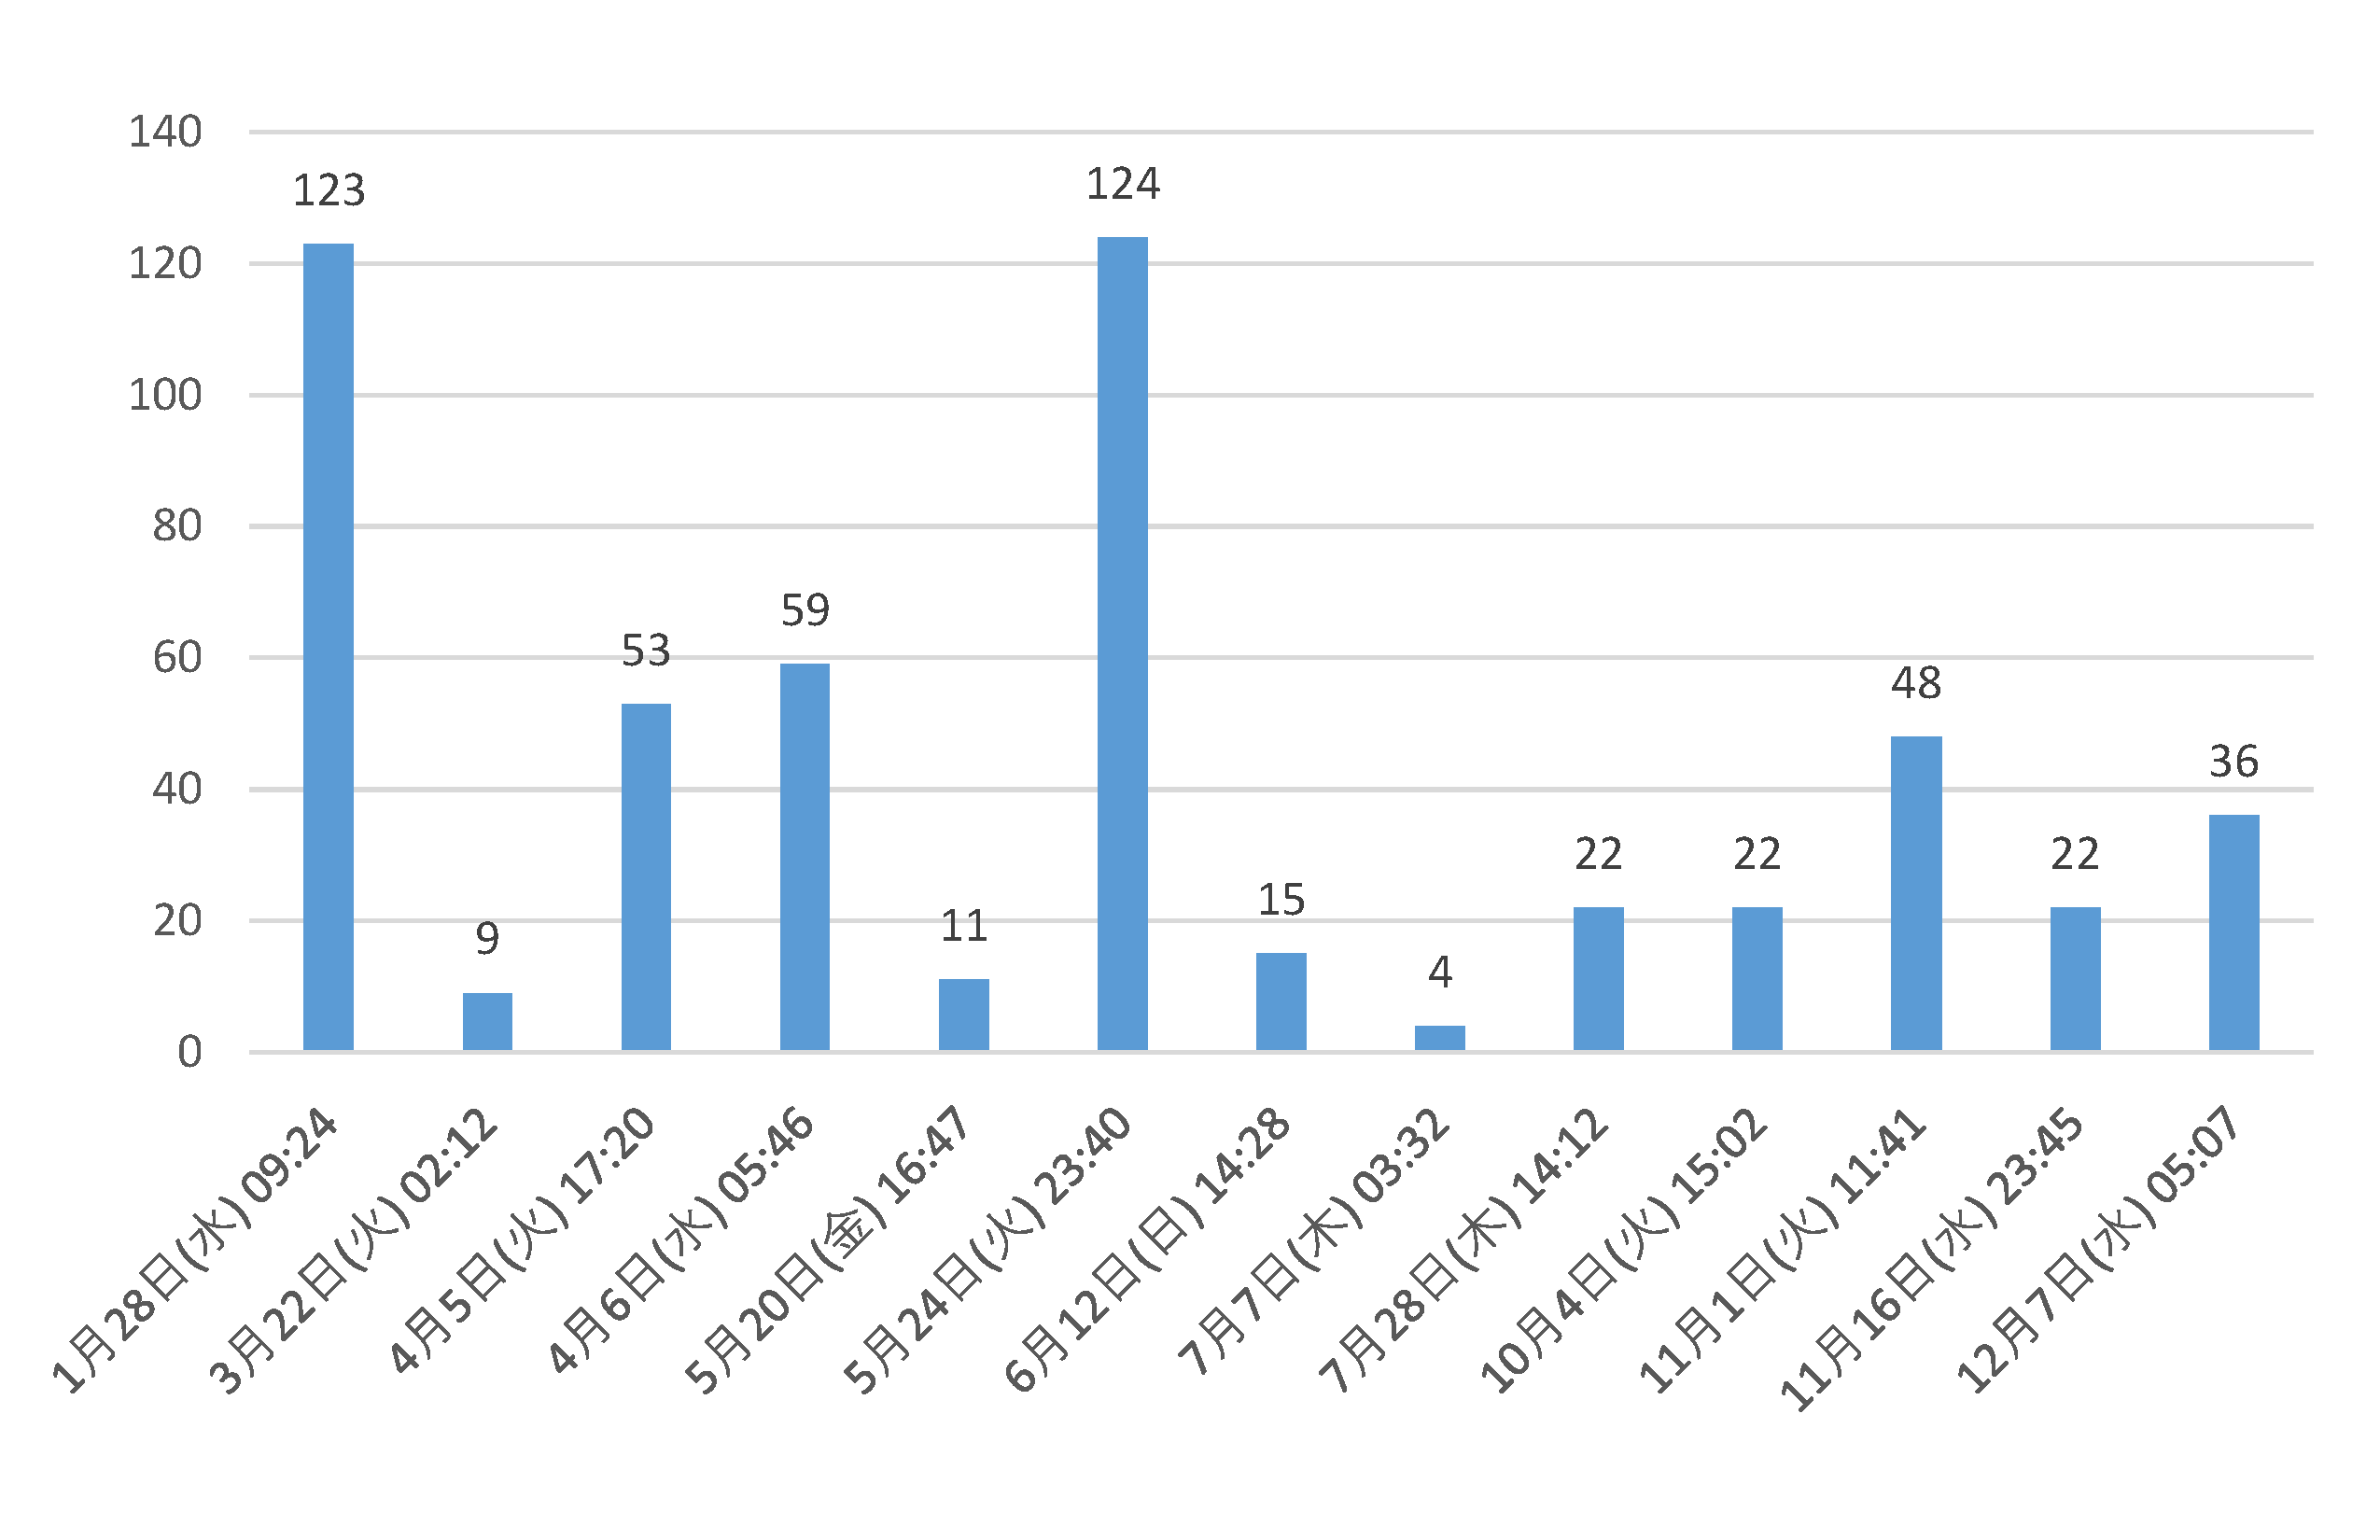
\includegraphics[width=8.4cm,clip]{graph1.pdf}
\caption{サービス停止から復旧までの間隔}\label{時間}
\end{figure}
\begin{figure}[H]
%\includegraphics[width=図の幅,clip]{ファイル名}\label{参照用ラベル}
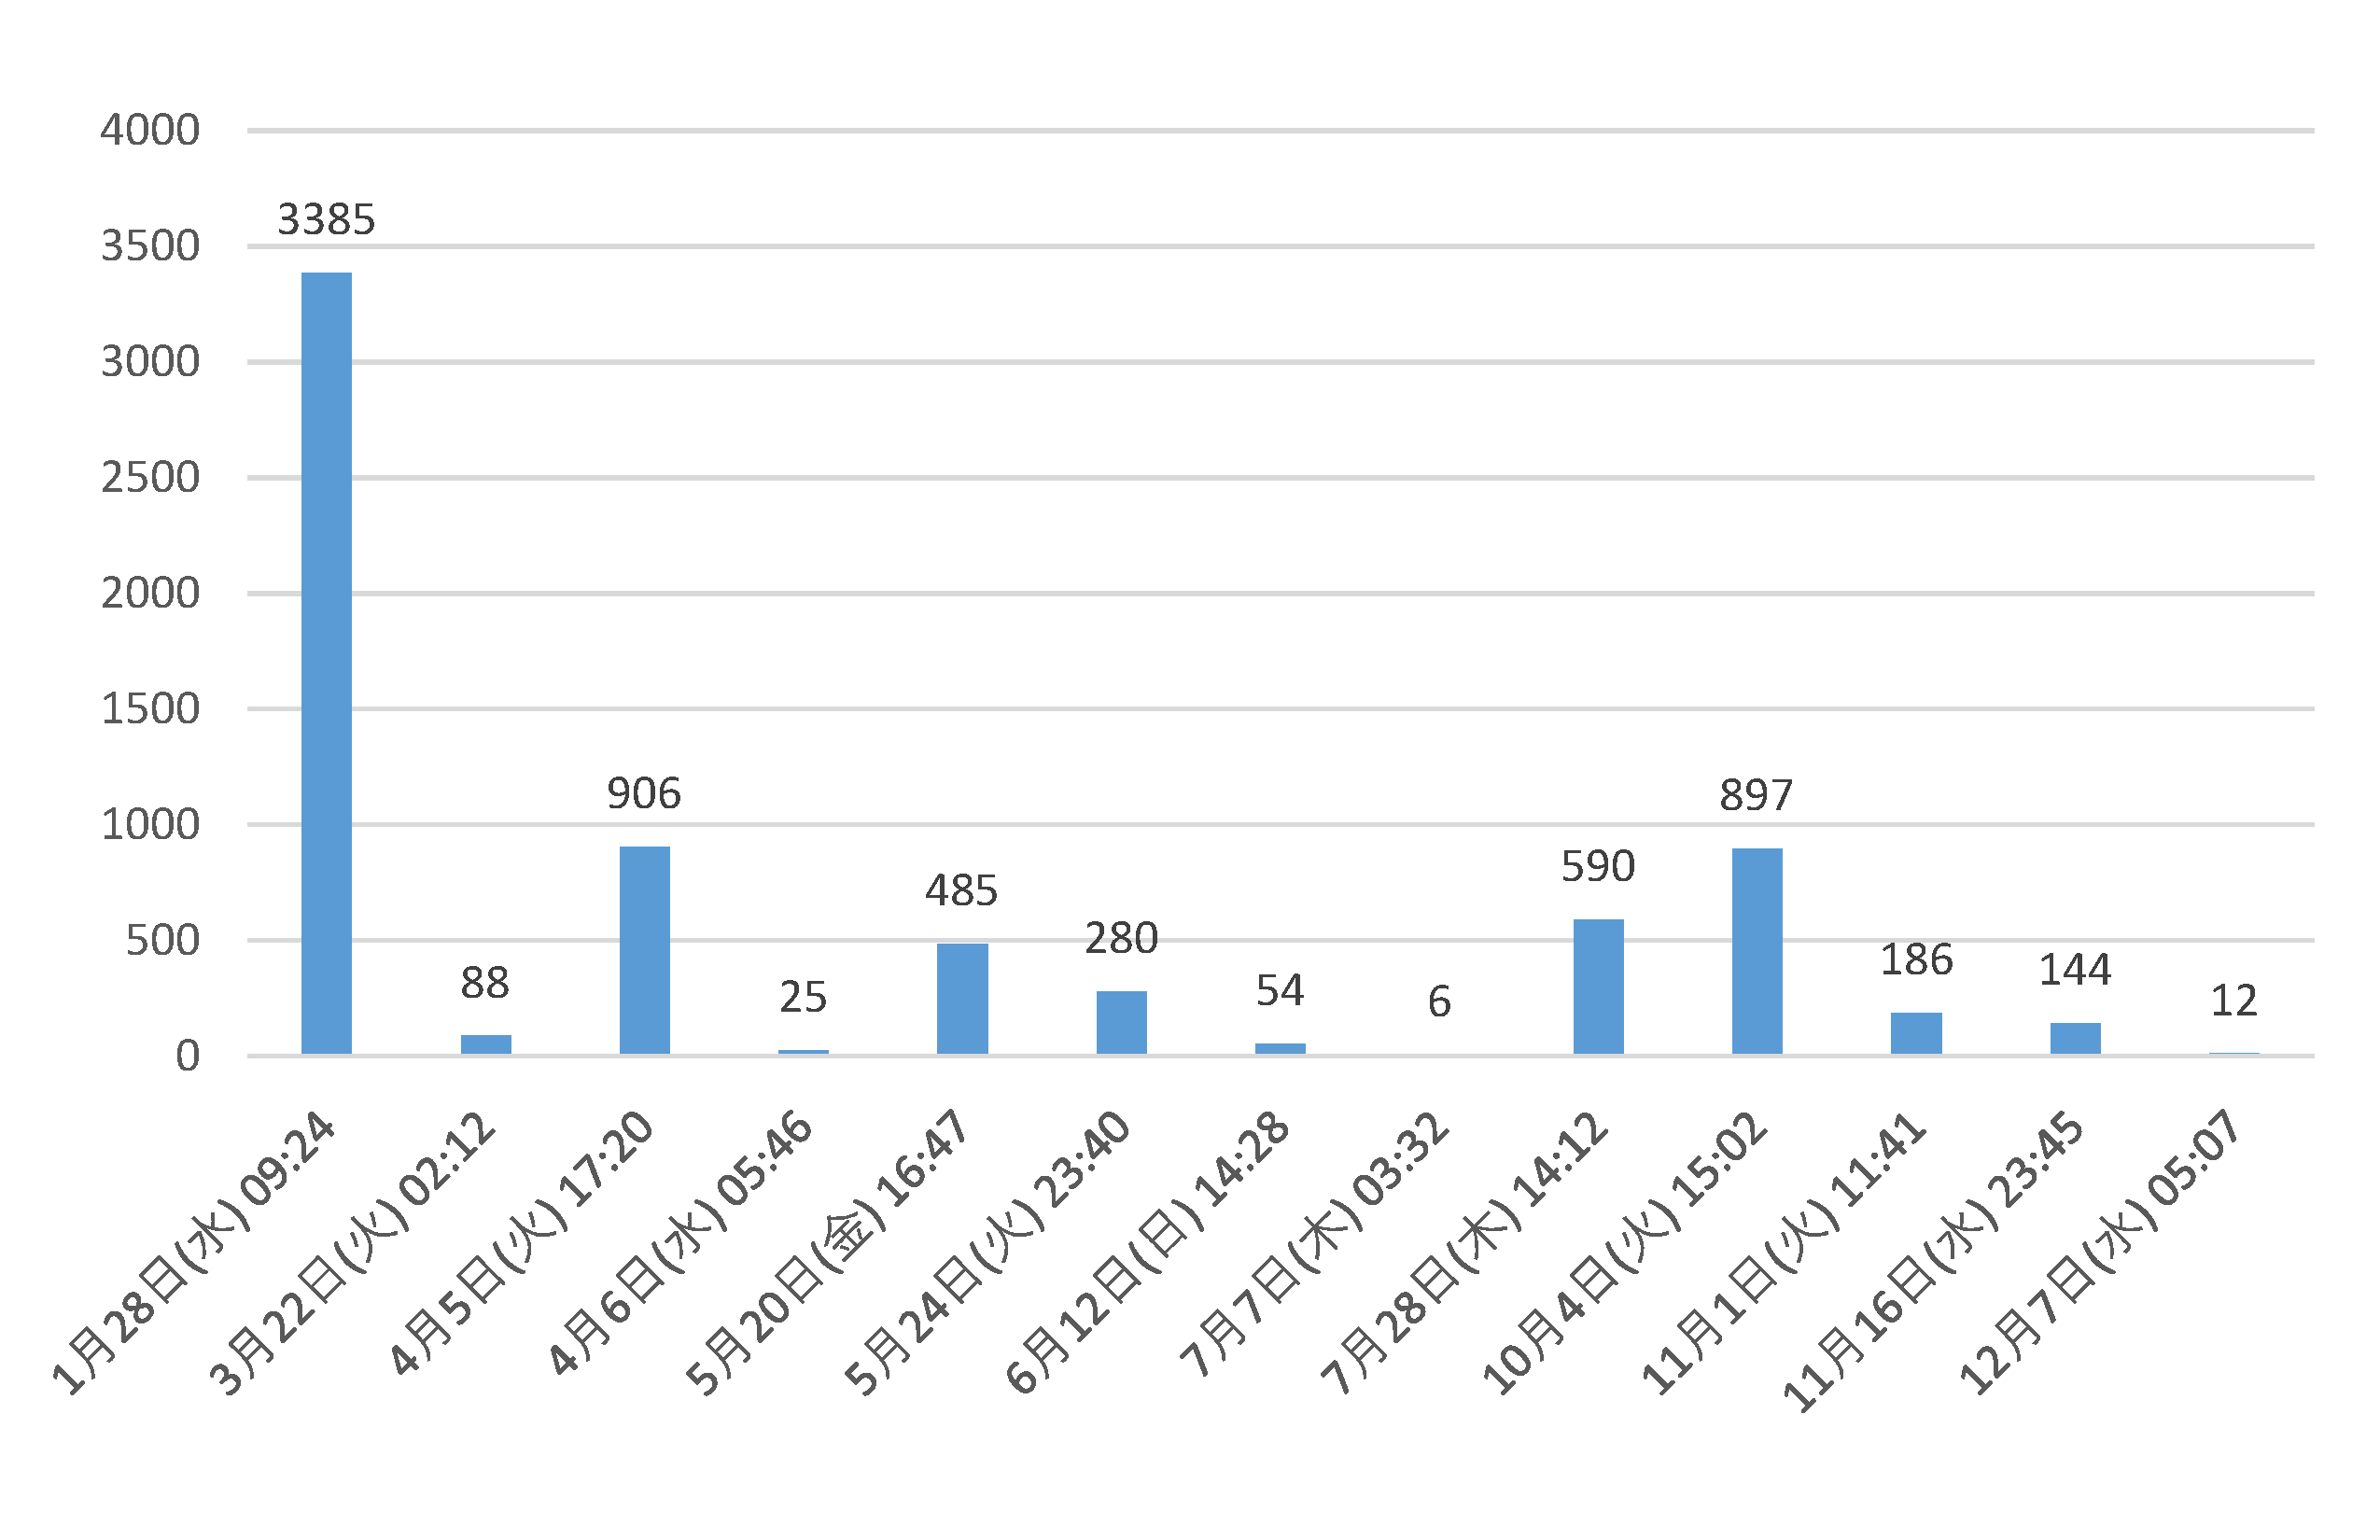
\includegraphics[width=8.4cm,clip]{graph2.pdf}
\caption{サービス停止中に投稿されたツイートの数}\label{ツイート数}
\end{figure}
13回分の各障害のサービス停止から復旧までの間隔を分単位でグラフにしたものが図\ref{時間}である.

そして,各障害のサービス停止中に投稿されたツイート数をグラフにしたものが図\ref{ツイート数}である.

\section{考察}
調査した13回分の障害を比較すると,サービス停止から復旧までの間隔が同じくらいでも,1日の時間帯によってツイート数に違いがあった.特にツイート数が多かったのは平日の日中で,中でも会社への出勤や退勤にあたる時間帯だった.この時間帯にWebサービスが停止してしまうと例え数分の停止でもツイート数が多く,1日のタスクが確認できなかったり,チーム内でのコミュニケーションが取れなかったりしてしまう.

平日の日中であればツイート数が多いのはもちろんだったが,3月22日(火)の深夜2時台に発生した約9分間の障害でも88件のツイートが集まった.日中の障害でも6月12日(日)と7月28日(木)では同じ14時台の障害で停止時間に約7分の差はあるが500ツイート以上の差があった.これは日曜日に起きた障害であり,普段仕事をしている人々が休暇中だったため少なかったのではないかと考えられる.

また,GitHub StatusのStatus Messageを参照してツイート取得する日を決定していたが,Status Messageに記されているサービス停止や復旧のアナウンスよりも,サービス停止や復旧したという旨のツイートの方が平均して約 8 分ほど早かった.これはTwitterの速報性が優れていると言える.

\section{結論}
本研究ではWebサービスの障害発生について調査した.Webサービスは利便性が高く,それだけに依存してしまうこともある.そのサービスが停止してしまうことは頻繁に有ることではなく,一時的なものだが,そのWebサービスを使用しているユーザーの仕事やコミュニケーションに少なからず影響を及ぼしてしまう.したがって,ソフトウェア開発プロジェクトなどでWebサービスを使用する場合は,サーバーダウン等の障害が発生するリスクを考慮する必要がある.

\bibliographystyle{junsrt}
\bibliography{biblio}%「biblio.bib」というファイルが必要.


\end{document}